
%%%%%%%%%%%%%%%%%%%%%%%%%%%%%%%%%%%%%%%%%%%%%%%%%%%%%%%%%%%%%%%%%%%%%%%%%%%%%%%%
%% ************************************************************************** %%
%% *                                Settings                                * %%
%% ************************************************************************** %%
%%%%%%%%%%%%%%%%%%%%%%%%%%%%%%%%%%%%%%%%%%%%%%%%%%%%%%%%%%%%%%%%%%%%%%%%%%%%%%%%
\documentclass{tron}

\loadglsentries{gls}
\glsaddall
\addbibresource{reference}
\usepackage{xcolor}  % Coloured text etc.
% fancy note style
% STYLE NOTES : v2.0
% additional fancy boxes
\usepackage[framemethod=TikZ]{mdframed}
%\usepackage{amsthm}

% gray color indicates [OPTIONAL READING]

%%%%%%%%%%%%%%%%%%%%%%%%%%%%%%
%Note
\newenvironment{note}[3][]{%
	\ifstrempty{#1}%
	{\mdfsetup{%
	frametitle={%
	\tikz[baseline=(current bounding box.east),outer sep=0pt]
	\node[anchor=east,rectangle,fill=#2]
	{\strut Note};}}
	}%
	{\mdfsetup{%
	frametitle={%
	\tikz[baseline=(current bounding box.east),outer sep=0pt]
	\node[anchor=east,rectangle,fill=#2]
	{\strut #1};}}%
	}%
	\mdfsetup{innertopmargin=0pt,skipabove=5pt,linecolor=#2,%
		linewidth=2pt,topline=true,%
		frametitleaboveskip=\dimexpr-\ht\strutbox\relax,
		backgroundcolor={white!90!#2}}
	\begin{mdframed}[]\relax%
	\label{#3}}{\end{mdframed}
}
\Crefname{note}{Note}{notes}

\newcommand{\createnoteenv}[6]{
	\refstepcounter{#6}%
	\ifstrempty{#1}%
	{\mdfsetup{%
	frametitle={%
	\tikz[baseline=(current bounding box.east),outer sep=0pt]
	\node[anchor=east,rectangle,fill=#3]
	{\strut #4~#5};}}
	}%
	{
		\mdfsetup{%
			frametitle={%
				\tikz[baseline=(current bounding box.east),outer sep=0pt]
				\node[anchor=east,rectangle,fill=#3]
				{\strut #4~#5:~#1};
			}
		}%
	}%
	\mdfsetup{innertopmargin=0pt,skipabove=5pt,linecolor=#3,%
	linewidth=2pt,topline=true,%
	frametitleaboveskip=\dimexpr-\ht\strutbox\relax,
	backgroundcolor={white!90!#3}}
	\begin{mdframed}[]\relax%
	\label{#2}
}

%%%%%%%%%%%%%%%%%%%%%%%%%%%%%%
%Definition
\newcounter{definition}[section] \setcounter{definition}{0}
\renewcommand{\thedefinition}{\arabic{section}.\arabic{definition}}
\newenvironment{definition}[2][]{%
	\createnoteenv{#1}{#2}{blue!40}{Definition}{\thedefinition}{definition}%
}{\end{mdframed}}
\newenvironment{definition*}[2][]{%
	\createnoteenv{#1}{#2}{gray!40}{Definition}{\thedefinition}{definition}%
}{\end{mdframed}}
\Crefname{definition}{Definition}{definitions}


%%%%%%%%%%%%%%%%%%%%%%%%%%%%%%
%theoremrem
\newcounter{theorem}[section] \setcounter{theorem}{0}
\renewcommand{\thetheorem}{\arabic{section}.\arabic{theorem}}
\newenvironment{theorem}[2][]{%
	\createnoteenv{#1}{#2}{cyan!40}{Theorem}{\thetheorem}{theorem}%
}{\end{mdframed}}
\newenvironment{theorem*}[2][]{%
	\createnoteenv{#1}{#2}{gray!40}{Theorem}{\thetheorem}{theorem}%
}{\end{mdframed}}
\Crefname{theorem}{Theorem}{theorems}

%%%%%%%%%%%%%%%%%%%%%%%%%%%%%%
%Proof
\newcounter{proof}[section]\setcounter{proof}{0}
\renewcommand{\theproof}{\arabic{section}.\arabic{proof}}
\newenvironment{proof}[2][]{%
	\createnoteenv{#1}{#2}{red!20}{Proof}{\theproof}{proof}%
}{\end{mdframed}}
\newenvironment{proof*}[2][]{%
	\createnoteenv{#1}{#2}{gray!40}{Proof}{\theproof}{proof}%
}{\end{mdframed}}
\Crefname{proof}{Proof}{proofs}


%%%%%%%%%%%%%%%%%%%%%%%%%%%%%%
%Alert
\newcounter{alert}[section]\setcounter{alert}{0}
\renewcommand{\thealert}{\arabic{section}.\arabic{alert}}
\newenvironment{alert}[2][]{%
	\createnoteenv{#1}{#2}{red!80}{Alert}{\thealert}{alert}%
}{\end{mdframed}}
\newenvironment{alert*}[2][]{%
	\createnoteenv{#1}{#2}{gray!40}{Alert}{\thealert}{alert}%
}{\end{mdframed}}
\Crefname{alert}{Alert}{alerts}

%%%%%%%%%%%%%%%%%%%%%%%%%%%%%%
%Answer
\newcounter{answer}[section]\setcounter{answer}{0}
\renewcommand{\theanswer}{\arabic{section}.\arabic{answer}}
\newenvironment{answer}[2][]{%
	\createnoteenv{#1}{#2}{orange!60}{Answer}{\theanswer}{answer}%
}{\end{mdframed}}
\newenvironment{answer*}[2][]{%
	\createnoteenv{#1}{#2}{gray!40}{Answer}{\theanswer}{answer}%
}{\end{mdframed}}
\Crefname{answer}{Answer}{answers}

%%%%%%%%%%%%%%%%%%%%%%%%%%%%%%
%Remark
\newcounter{remark}[section]\setcounter{remark}{0}
\renewcommand{\theremark}{\arabic{section}.\arabic{remark}}
\newenvironment{remark}[2][]{%
	\createnoteenv{#1}{#2}{orange!40}{Remark}{\theremark}{remark}%
}{\end{mdframed}}
\newenvironment{remark*}[2][]{%
	\createnoteenv{#1}{#2}{gray!40}{Remark}{\theremark}{remark}%
}{\end{mdframed}}
\Crefname{remark}{Remark}{remarks}


%%%%%%%%%%%%%%%%%%%%%%%%%%%%%%%
%%Example
%\newcounter{example}[section]\setcounter{example}{0}
%\renewcommand{\theexample}{\arabic{section}.\arabic{example}}
%\newenvironment{example}[2][]{%
%	\createnoteenv{#1}{#2}{blue!40!cyan!20}{Example}{\theexample}{example}%
%}{\end{mdframed}}
%\newenvironment{example*}[2][]{%
%	\createnoteenv{#1}{#2}{gray!40}{Example}{\theexample}{example}%
%}{\end{mdframed}}

%%%%%%%%%%%%%%%%%%%%%%%%%%%%%%
%Algorithm
\newcounter{algo}[section]\setcounter{algo}{0}
\renewcommand{\thealgo}{\arabic{algo}.\arabic{algo}}
\newenvironment{algo}[2][]{%
	\createnoteenv{#1}{#2}{yellow!90!brown!60}{Algorithm}{\thealgo}{algo}%
}{\end{mdframed}}
\newenvironment{algo*}[2][]{%
	\createnoteenv{#1}{#2}{gray!40}{Algorithm}{\thealgo}{algo}%
}{\end{mdframed}}
\Crefname{algo}{Algorithm}{algos}

%%%%%%%%%%%%%%%%%%%%%%%%%%%%%%
% CS480 - Exercise
%\setlength{\parskip}{1cm}
%\setlength{\parindent}{1cm}

%\tikzstyle{titregris} =
%[draw=gray,fill=white, shading = exersicetitle, %
%text=gray, rectangle, rounded corners, right,minimum height=.3cm]
%\pgfdeclarehorizontalshading{exersicebackground}{100bp}
%{color(0bp)=(green!40); color(100bp)=(black!5)}
%\pgfdeclarehorizontalshading{exersicetitle}{100bp}
%{color(0bp)=(red!40);color(100bp)=(black!5)}
%\newcounter{exercise}
%\renewcommand*\theexercise{exercice \textbf{Exercice}~n\arabic{exercise}}
%\makeatletter
%\def\mdf@@exercisepoints{}%new mdframed key:
%\define@key{mdf}{exercisepoints}{%
%\def\mdf@@exercisepoints{#1}
%}
%
%\mdfdefinestyle{theoremstyle}{%
%outerlinewidth=0.01em,linecolor=black,middlelinewidth=0.5pt,%
%frametitlerule=true,roundcorner=2pt,%
%apptotikzsetting={\tikzset{mfframetitlebackground/.append style={%
%shade,left color=white, right color=blue!20}}},
%frametitlerulecolor=black,innertopmargin=1\baselineskip,%green!60,
%innerbottommargin=0.5\baselineskip,
%frametitlerulewidth=0.1pt,
%innertopmargin=0.7\topskip,skipabove={\dimexpr0.2\baselineskip+0.1\topskip\relax},
%frametitleaboveskip=1pt,
%frametitlebelowskip=1pt
%}
%\mdtheorem[style=theoremstyle]{exercise}{\textbf{Exercise}}

\newcounter{exercise}[section]\setcounter{exercise}{0}
\renewcommand{\theexercise}{\arabic{exercise}}
\newenvironment{exercise}[2][]{%
	\createnoteenv{#1}{#2}{gray!40}{Exercise}{\theexercise}{exercise}%
}{\end{mdframed}}
\newenvironment{exercise*}[2][]{%
	\createnoteenv{#1}{#2}{gray!40}{Exercise}{\theexercise}{exercise}%
}{\end{mdframed}}

\Crefname{exercise}{Exercise}{exercises}


%%%%%%%%%%%%%%%%%%%%%%%%%%%%%%
%Examples
% {

%     \section{Theorem and lemma examples with title}
%     \begin{theorem}[Pythagoras' theorem]{theorem:pythagoras}
%     In a right triangle, the square of the hypotenuse is equal to the sum of the squares of the catheti.
%     \[a^2+b^2=c^2\]
%     \end{theorem}
%     In mathematics, the Pythagorean theorem, also known as Pythagoras' theorem (see theorem \ref{theorem:pythagoras}), is a relation in Euclidean geometry among the three sides of a right triangle.
%     
%     \begin{definition}[B\'ezout's identity]{def:bezout}
%     Let $a$ and $b$ be nonzero integers and let $d$ be their greatest common divisor. Then there exist integers $x$ and $y$ such that:
%     \[ax+by=d\]
%     \end{definition}
%     This is a reference to Bezout's lemma \ref{def:bezout}
%     
%     
%     \section{Theorem and proof examples without title}
%     
%     \begin{theorem}[]{theorem:theorem1}
%     There exist two irrational numbers $x$, $y$ such that $x^y$ is rational.
%     \end{theorem}
%     
%     \begin{proof}[]{proof:proof1}
%     If $x=y=\sqrt{2}$ is an example, then we are done; otherwise $\sqrt{2}^{\sqrt{2}}$ is irrational, in which case taking $x=\sqrt{2}^{\sqrt{2}}$ and $y=\sqrt{2}$ gives us:
%     \[\bigg(\sqrt{2}^{\sqrt{2}}\bigg)^{\sqrt{2}}=\sqrt{2}^{\sqrt{2}\sqrt{2}}=\sqrt{2}^{2}=2.\]
%     \end{proof}
%
%     \begin{alert}[]{alert:alert1}
%     If $x=y=\sqrt{2}$ is an example, then we are done; otherwise $\sqrt{2}^{\sqrt{2}}$ is irrational, in which case taking $x=\sqrt{2}^{\sqrt{2}}$ and $y=\sqrt{2}$ gives us:
%     \[\bigg(\sqrt{2}^{\sqrt{2}}\bigg)^{\sqrt{2}}=\sqrt{2}^{\sqrt{2}\sqrt{2}}=\sqrt{2}^{2}=2.\]
%     \end{alert}
%     
%     \begin{remark}[]{alert:alert1}
%     If $x=y=\sqrt{2}$ is an example, then we are done; otherwise $\sqrt{2}^{\sqrt{2}}$ is irrational, in which case taking $x=\sqrt{2}^{\sqrt{2}}$ and $y=\sqrt{2}$ gives us:
%     \[\bigg(\sqrt{2}^{\sqrt{2}}\bigg)^{\sqrt{2}}=\sqrt{2}^{\sqrt{2}\sqrt{2}}=\sqrt{2}^{2}=2.\]
%     \end{remark}
%     
%     
%          \begin{exercise}[]{alert:alert1}
%     If $x=y=\sqrt{2}$ is an example, then we are done; otherwise $\sqrt{2}^{\sqrt{2}}$ is irrational, in which case taking $x=\sqrt{2}^{\sqrt{2}}$ and $y=\sqrt{2}$ gives us:
%     \[\bigg(\sqrt{2}^{\sqrt{2}}\bigg)^{\sqrt{2}}=\sqrt{2}^{\sqrt{2}\sqrt{2}}=\sqrt{2}^{2}=2.\]
%     \end{exercise}
%     
%     \begin{algo}[]{algorithm:alert1}
%     If $x=y=\sqrt{2}$ is an example, then we are done; otherwise $\sqrt{2}^{\sqrt{2}}$ is irrational, in which case taking $x=\sqrt{2}^{\sqrt{2}}$ and $y=\sqrt{2}$ gives us:
%     \[\bigg(\sqrt{2}^{\sqrt{2}}\bigg)^{\sqrt{2}}=\sqrt{2}^{\sqrt{2}\sqrt{2}}=\sqrt{2}^{2}=2.\]
%     \end{algo}
%     
%     \begin{note}[Goal]{pink}{note:goal}
%     If $x=y=\sqrt{2}$ is an example, then we are done; otherwise $\sqrt{2}^{\sqrt{2}}$ is irrational, in which case taking $x=\sqrt{2}^{\sqrt{2}}$ and $y=\sqrt{2}$ gives us:
%     \[\bigg(\sqrt{2}^{\sqrt{2}}\bigg)^{\sqrt{2}}=\sqrt{2}^{\sqrt{2}\sqrt{2}}=\sqrt{2}^{2}=2.\]
%     \end{note}

% }
%\usepackage{lipsum}                     % Dummytext
\usepackage{xargs}                      % Use more than one optional parameter in a new commands
\usepackage[colorinlistoftodos,prependcaption,textsize=normalsize]{todonotes}
%
\newcommandx{\unsure}[2][1=]{\todo[linecolor=red,backgroundcolor=red!25,bordercolor=red,#1]{#2}}
\newcommandx{\change}[2][1=]{\todo[linecolor=blue,backgroundcolor=blue!25,bordercolor=blue,#1]{#2}}
\newcommandx{\info}[2][1=]{\todo[linecolor=OliveGreen,backgroundcolor=OliveGreen!25,bordercolor=OliveGreen,#1]{#2}}
\newcommandx{\improvement}[2][1=]{\todo[linecolor=Plum,backgroundcolor=Plum!25,bordercolor=Plum,#1]{#2}}
\newcommandx{\thiswillnotshow}[2][1=]{\todo[disable,#1]{#2}}
%
\preto\printlistoftodos{
    \listoftodos[Todo List]
}

% EXAMPLES:
    % \todo[inline]{The original todo note withouth changed colours.\newline Here's another line.}
    % \lipsum[11]\unsure{Is this correct?}\unsure{I'm unsure about also!}
    % \lipsum[11]\change{Change this!}
    % \lipsum[11]\info{This can help me in chapter seven!}
    % \lipsum[11]\improvement{This really needs to be improved!\newline\newline What was I thinking?!}
    % \lipsum[11]
    % \thiswillnotshow{This is hidden since option `disable' is chosen!}
    % \improvement[inline]{The following section needs to be rewritten!}
    % \lipsum[11]
    % \newpage
    % \listoftodos[Notes]
%%%  Equation Condition
\newenvironment{eqconditions}
  {\par\vspace{\abovedisplayskip}\noindent\begin{tabular}{>{$}l<{$} @{${}={}$} l}}
  {\end{tabular}\par\vspace{\belowdisplayskip}}
\newenvironment{eqconditions*}
  {\noindent\begin{tabular}{>{$}l<{$} @{${}={}$} l}}
  {\end{tabular}}
%%% introduce 4th depth with \paragraph command
\usepackage{titlesec}
\setcounter{secnumdepth}{4}
\titleformat{\paragraph}
{\normalfont\normalsize\bfseries}{\theparagraph}{1em}{}
\titlespacing*{\paragraph}
{0pt}{3.25ex plus 1ex minus .2ex}{1.5ex plus .2ex}

%%% enumeration reference
% constraint
\newlist{constraint-list}{enumerate}{1}
\setlist[constraint-list,1]{leftmargin=*, label= \Roman*}
\creflabelformat{Constraint}{#2#1#3}
\crefname{constraint-listi}{Constraint}{position}
% criteria
\newlist{criteria-list}{enumerate}{1}
\setlist[criteria-list,1]{leftmargin=*, label= \Roman*}
\creflabelformat{Criterion}{#2#1#3}
\crefname{criteria-listi}{Criterion}{position}
% property
\newlist{property-list}{enumerate}{1}
\setlist[property-list,1]{leftmargin=*, label= \Roman*}
\creflabelformat{Property}{#2#1#3}
\crefname{property-listi}{Property}{position}
% assumption
\newlist{assumption-list}{enumerate}{1}
\setlist[assumption-list,1]{leftmargin=*, label= \Roman*}
\creflabelformat{Assumption}{#2#1#3}
\crefname{assumption-listi}{Assumption}{position}

% custom math command
\newcommand{\unit}[1]{\left[\si{#1}\right]}

% additional math packages
\usepackage{physics}
\usepackage{cancel}

% TODO Flags
\newcommand\TODO[1]{{\textcolor{red}{\textbf{#1}}}}
\newcommand\COMMENT[1]{\hl{#1}}

% Custom Format
% \usepackage{float}
% \usepackage[table]{xcolor}
% \usepackage{soul}
\usepackage{multirow}
\usepackage{caption} 
\captionsetup[table]{skip=3pt}
\captionsetup[figure]{skip=0pt}
\titlespacing*{\section}
{0pt}{10pt}{3pt}
\titlespacing*{\subsection}
{0pt}{8pt}{3pt}
\titlespacing*{\subsubsection}
{0pt}{8pt}{3pt}
%hide the highlight box
\hypersetup{
    colorlinks,
    linkcolor={black!50!black},
    citecolor={black!50!blue},
    urlcolor={black!80!black}
}%hide the highlight box

% table formatting
% \setlength{\arrayrulewidth}{1mm}
% \setlength{\tabcolsep}{18pt}
% \renewcommand{\arraystretch}{2.5}
\usepackage{array}
\newcolumntype{C}[1]{>{\centering\let\newline\\\arraybackslash\hspace{0pt}}m{#1}}

% custom math symbol
%% CS 480 %%
\newcommand{\bm}[1]{\mathbf{#1}}
%%%%%%%%%%%%
\newcommand{\RR}{\mathds{R}}
\newcommand{\Id}{\mathbb{I}}
\newcommand{\NN}{\mathds{N}}
\newcommand{\sign}{\mathop{\mathrm{sign}}}
\newcommand{\diag}{\mathop{\mathrm{diag}}}
\newcommand{\argmin}{\mathop{\mathrm{argmin}}}
\newcommand{\zero}{\mathbf{0}}
\newcommand{\one}{\mathbf{1}}
\newcommand{\av}{\mathbf{a}}
\newcommand{\bv}{\mathbf{b}}
\newcommand{\sv}{\mathbf{s}}
\newcommand{\Xv}{\mathbf{X}}
\newcommand{\Yv}{\mathbf{Y}}
\newcommand{\wv}{\mathbf{w}}
\newcommand{\xv}{\mathbf{x}}
\newcommand{\yv}{\mathbf{y}}
\newcommand{\zv}{\mathbf{z}}
\newcommand{\uv}{\mathbf{u}}
\newcommand{\rv}{\mathbf{r}}
\newcommand{\inner}[2]{\langle #1, #2 \rangle}
\newcommand{\red}[1]{{\color{red}#1}}
\newcommand{\blue}[1]{{\color{blue}#1}}
\newcommand{\magenta}[1]{{\color{magenta}#1}}


\newcommand{\ea}{{et al.}\xspace}
\newcommand{\eg}{{e.g.}\xspace}
\newcommand{\ie}{{i.e.}\xspace}
\newcommand{\iid}{{i.i.d.}\xspace}
\newcommand{\cf}{{cf.}\xspace}
\newcommand{\wrt}{{w.r.t.}\xspace}
\newcommand{\aka}{{a.k.a.}\xspace}
\newcommand{\etc}{{etc.}\xspace}
\newcommand{\sgm}{\mathsf{sgm}}
\newcommand{\Dc}{\mathcal{D}}
\newcommand{\ans}[1]{{\textcolor{orange}{\textsf{Ans}: #1}}}



\usepackage{float}
% extra mod
\newcommand{\mref}[1]{\underline{\textbf{\hypersetup{linkcolor=orange}\Cref{#1}\hypersetup{linkcolor=blue}}}}

%%%%%%%%%%%%%%%%%%%%%%%%%%%%%%%%%%%%%%%%%%%%%%%%%%%%%%%%%%%%%%%%%%%%%%%%%%%%%%%%
% Make sure the following block contains the correct information               %
%%%%%%%%%%%%%%%%%%%%%%%%%%%%%%%%%%%%%%%%%%%%%%%%%%%%%%%%%%%%%%%%%%%%%%%%%%%%%%%%
\reporttitle{ECE 488 - Project 3 \& 4}
% \selfstudy % comment this line if this is not a self study report 
% \employername{Employer Name}
% \employerstreetaddress{Employer Address}
% \employerlocation{City, Provice, Country}
\university{University of Waterloo}
\faculty{Faculty of Engineering}%Faculty of Engineering
\department{}%Department of Systems Design Engineering
\groupnumber{1}
\authornameA{Jianxiang (Jack) Xu}
\studentnumberA{20658861}
\reportdate{\today}
%\confidential{1} % comment this line if this is not a confidential report
%\authorstreetaddress{##}
%\authorlocation{##}
%\authorpostalcode{##}
\useheader % comment this line if no need for header
%%%%%%%%%%%%%%%%%%%%%%%%%%%%%%%%%%%%%%%%%%%%%%%%%%%%%%%%%%%%%%%%%%%%%%%%%%%%%%%%
% end of information block...                                                  %
%%%%%%%%%%%%%%%%%%%%%%%%%%%%%%%%%%%%%%%%%%%%%%%%%%%%%%%%%%%%%%%%%%%%%%%%%%%%%%%%

\begin{document}
%%%%%%%%%%%%%%%%%%%%%%%%%%%%%%%%%%%%%%%%%%%%%%%%%%%%%%%%%%%%%%%%%%%%%%%%%%%%%%%%
%% ************************************************************************** %%
%% *                               Title Page                               * %%
%% ************************************************************************** %%
%%%%%%%%%%%%%%%%%%%%%%%%%%%%%%%%%%%%%%%%%%%%%%%%%%%%%%%%%%%%%%%%%%%%%%%%%%%%%%%%
\maketitle
%%%%%%%%%%%%%%%%%%%%%%%%%%%%%%%%%%%%%%%%%%%%%%%%%%%%%%%%%%%%%%%%%%%%%%%%%%%%%%%%
%% ************************************************************************** %%
%% *                           Table of Contents                            * %%
%% ************************************************************************** %%
%%%%%%%%%%%%%%%%%%%%%%%%%%%%%%%%%%%%%%%%%%%%%%%%%%%%%%%%%%%%%%%%%%%%%%%%%%%%%%%%
 \tableofcontents
%%%%%%%%%%%%%%%%%%%%%%%%%%%%%%%%%%%%%%%%%%%%%%%%%%%%%%%%%%%%%%%%%%%%%%%%%%%%%%%%
%% ************************************************************************** %%
%% *                            List of Figures                             * %%
%% ************************************************************************** %%
%%%%%%%%%%%%%%%%%%%%%%%%%%%%%%%%%%%%%%%%%%%%%%%%%%%%%%%%%%%%%%%%%%%%%%%%%%%%%%%%
% \listoffigures
%%%%%%%%%%%%%%%%%%%%%%%%%%%%%%%%%%%%%%%%%%%%%%%%%%%%%%%%%%%%%%%%%%%%%%%%%%%%%%%%
%% ************************************************************************** %%
%% *                             List of Tables                             * %%
%% ************************************************************************** %%
%%%%%%%%%%%%%%%%%%%%%%%%%%%%%%%%%%%%%%%%%%%%%%%%%%%%%%%%%%%%%%%%%%%%%%%%%%%%%%%%
% \listoftables
%%%%%%%%%%%%%%%%%%%%%%%%%%%%%%%%%%%%%%%%%%%%%%%%%%%%%%%%%%%%%%%%%%%%%%%%%%%%%%%%
%% ************************************************************************** %%
%% *                              MAIN BODY                                 * %%
%% ************************************************************************** %%
%%%%%%%%%%%%%%%%%%%%%%%%%%%%%%%%%%%%%%%%%%%%%%%%%%%%%%%%%%%%%%
\clearpage
\pagenumbering{arabic}
\setcounter{page}{1}
\setlength{\parskip}{5pt}
\newpage

%%%%%%%%%%%%%%%%%%%%%%%%%%%%%%%%%%%
%%%%% Intro.  %%%%%%
%%%%%%%%%%%%%%%%%%%%%%%%%%%%%%%%%%%

%%%%%%%%%%%%%%%%
%%%%% Ex 1 %%%%%
%%%%%%%%%%%%%%%%
\section{Problem P3: Controller Design by Youla Parameterization for the SISO aiming system}
%\vspace{5pt}

% --- ANS (a) --- %
\subsection{(a) Controller Design $C_1(s)$ with Youla Parameterization \label{ans:P1-a}}
In order to achieve perfect steady-state tracking of steps, the final $C_1(s)$ must have an integrator in it. To achieve this, we may augment the plant with an integrator term (\Cref{eqn:p1-aug}), and design an augmented controller $C_1^{aug}(s)$ for the augmented plant $P_1^{aug}(s)$ through Youla Parameterization.
\begin{equation}
\label{eqn:p1-aug}
	P_1^{aug}(s) = \frac1s \, P_1(s) = \frac{8}{s\,(s-4.427)\,(s+4.427)}
\end{equation}
 
To perform Youla Parameterization, coprime factorization is performed with a scale factor of 10 to avoid numerical issues. The resultant coprimes can be found below:
\begin{align}
	M(s)  &= \frac{s (s-4.427) (s+4.427) }{ (s+30) (s+20) (s+10)} \\
	N(s)  &= \frac{ 8 }{ (s+30) (s+20) (s+10)} \\
	X(s)  &= \frac{ 255510 (s^2 + 7.861s + 17.61)}{ (s+30) (s+20) (s+10)} \\
	Y(s)  &= \frac{ (s+65.16) (s^2 + 54.84s + 2246) }{ (s+30) (s+20) (s+10)}
\end{align}
 
 For simplicity, we assume the $Q(s) = 1$, which may result a complex augmented controller:
 \begin{equation}
 	C_1^{aug}(s) = \frac{(s+255500) (s^2 + 7.861s + 17.61) }{ (s+65.15) (s^2 + 54.85s + 2246)}
 \end{equation}
 
 We may now obtain the final controller by applying the integrator term to the augmented controller obtained just now:
 \begin{equation}
 	C_1(s) = \frac1s \, C_1^{aug}(s) = \frac{(s+255500) (s^2 + 7.861s + 17.61) }{ s (s+65.15) (s^2 + 54.85s + 2246)}
 \end{equation}
 
The detailed implementation can be found in \Cref{code:main}.
 
 
\newpage
% --- ANS (b) --- %
\subsection{(b) Closed-loop step response for controller designed in \Cref{ans:P1-a} \label{ans:P1-b}}
We may now run the simulation with a step input of $0.5 \unit{rad}$ same as the Lab 1 and Lab 2. We may find the closed-loop system is indeed stable and the steady-state tracking error is zero from \Cref{fig:unit-step} below.

\begin{figure}[H]
	\centering
	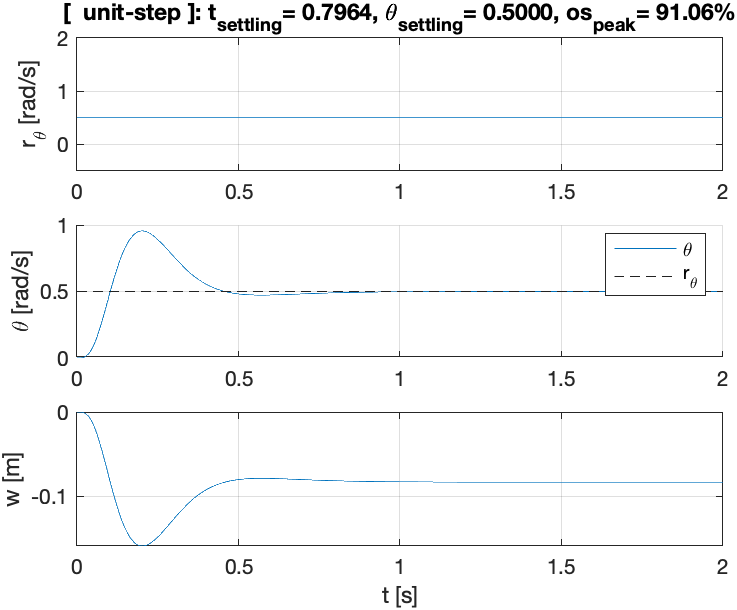
\includegraphics[height=250px]{../matlab/output/p3/step_response_unit-step}
	\caption{Closed-loop step response for controller $C_1(s)$ designed in \Cref{ans:P1-a}}
	\label{fig:unit-step}
\end{figure}

%How are the transients of your controller? 
As expected, a simple $Q(s)=1$ results a stable system, but there is no guarantee on the transient performance. From the \Cref{fig:unit-step}, we may observe a $91\%$ overshoot and $0.7964\unit{s}$ settling time. The overshoot is quite significant. 

To further analyze the system, a bode plot is generated for the closed-loop system, as shown in \Cref{fig:bode} below.

\begin{figure}[H]
	\centering
	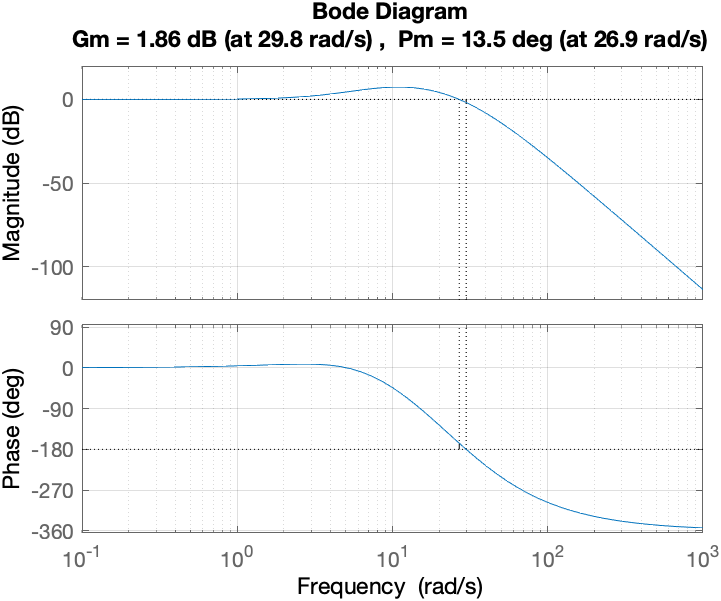
\includegraphics[height=250px]{../matlab/output/p3/bode_plot_r2theta}
	\caption{Bode plot for the closed-loop system designed in \Cref{ans:P1-a}}
	\label{fig:bode}
\end{figure}

From \Cref{fig:bode}, both gain margin ($1.86 \unit{dB}$) and phase margin ($13.5\unit{deg}$) are extremely small, hence the system is quite sensitive to noise and disturbances. To improve the transients and phase margin, we can adjust the parameter $Q(s)$ such that the desired criterion is met. Based on the research, many system utilizes Youla Parameterization with stochastic gradient descent, graph theory, and genetic algorithm to improve the transient performance by manipulating the $Q(s)$. Since, any proper transfer function of $Q(s)$ would result a stable controller from the Youla formulation, hence, all we need to do is to adaptively find the optimal solution via various adaptive and un-supervised learning approach.

%What is the phase margin? 
%Do you have insight into how to modify 𝑄𝑄 ( 𝑠𝑠 ) to improve the transients or phase margin? 
%[You like have zero intuition, demonstrating the point that design in the 𝑄𝑄 ( 𝑠𝑠 ) domain, although conceptually appealing and great for some computer-aided design techniques, has a major limitation.]

%\newpage
% --- ANS (c) --- %
\subsection{(c) [Optional] Simulation Visualization \label{ans:P1-c}}
The performance of the controller is visualized with the provided simulation, as shown in \Cref{fig:sim} below.
\begin{figure}[H]
	\centering
	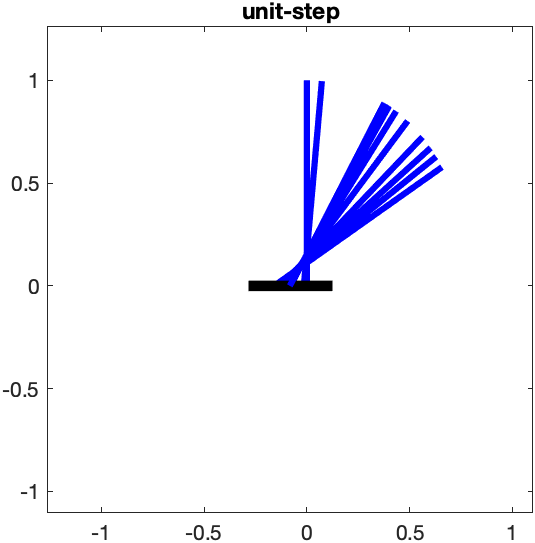
\includegraphics[height=250px]{../matlab/output/p3/sim_unit-step}
	\caption{Final simulation result of a unit-step response for the closed-loop system designed in \Cref{ans:P1-a}}
	\label{fig:sim}
\end{figure}


%%%%%%%%%%%%%%%%
%%%%% Ex 2 %%%%%
%%%%%%%%%%%%%%%%
\newpage
\section{Problem 4: Performance limitations associated with the SISO aiming system}
%\vspace{5pt}

% --- ANS (a) --- %
\subsection{(a) Performance limitations of one-rod system}
% --- ANS (a:i) --- %
\subsubsection{(i) Overshoot $y_{os}$ bound \label{sec:4ai}}
%We established that, because of the unstable plant pole, we need high bandwidth (i.e., a fast response) to get good performance. Assuming that integral control is used to get perfect steady-state step tracking, plot a curve that shows, as a function of rise time (𝑡𝑡 𝑟𝑟 ), a minimum bound on the closed-loop step response overshoot ( 𝑦𝑦 OS ). Assume a 1-DOF topology.

For a unit-step of $0.5 \unit{rad/s}$, the overshoot bound can be formulated in \Cref{eqn:p4:yos:bound}, and its corresponding bounding curve can be seen in \Cref{fig:yos} below.
\begin{equation}
	y_{os} \geq (1-0.9\, y_{\infty})(e^{p\, t_r} - 1) > 0 \label{eqn:p4:yos:bound}
\end{equation}
\begin{figure}[H]
	\centering
	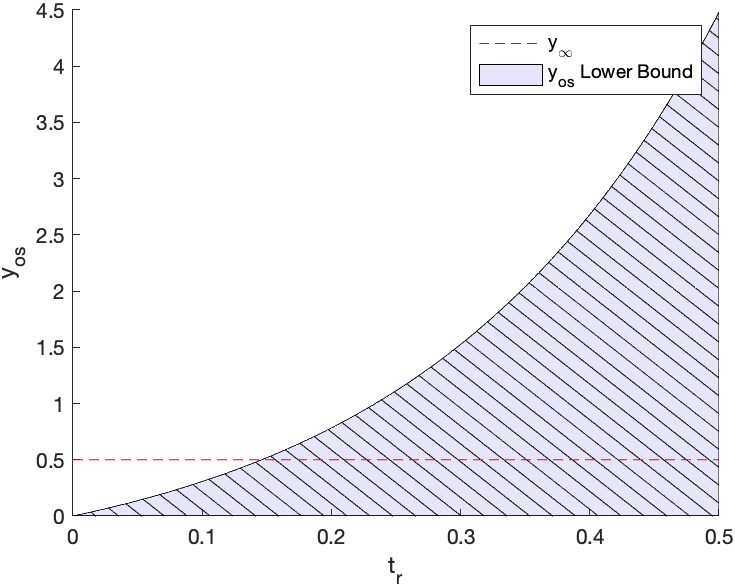
\includegraphics[height=250px]{../matlab/output/p4/y_os-bound}
	\caption{Overshoot $y_{os}$ bound}
	\label{fig:yos}
\end{figure}


\newpage
% --- ANS (a:ii) --- %
\subsubsection{(ii) $\Omega$ bound \label{sec:4aii}}
Three additional design specifications are imposed:
\begin{spec-list}
	\item For tracking performance, $|S(j\omega)| \leq -20 \unit{dB}$ for $\omega \in [0, 0.1] \unit{rad/s}$ \label{spec:track}
	\item For robust stability, $\underset{\omega}{\max}|S(j\omega)| \leq 5 \unit{dB}$ \label{spec:max}
	\item "Shut off" $\forall \omega > \Omega \unit{rad/s}$ \label{spec:shut}
\end{spec-list}

Since the controller stabilizes the closed loop system, and the loop gain has a relative degree of at least 2, the \Gls{BSI} (Bode Sensitivity Integral) holds. We may now derive the $Omega$ boundary (\Cref{eqn:omega:bnd}) from the \Gls{BSI} inequality for the sensitivity function, as derived below:
\begin{align}
	\int_0^{\infty} \ln |S(j\omega)| d\omega 	& = \pi \cdot \sum_{i=1}^{N_p} \Re(p_i) \\
\text{\Cref{spec:shut} \& \Cref{spec:track}} \Rightarrow \quad 	\int_0^{0.1} \ln |S(j\omega)| d\omega + \int_{0.1}^{\Omega} \ln |S(j\omega)| d\omega & \geq \pi \cdot \sum_{i=1}^{N_p} \Re(p_i) \\
\text{\Cref{spec:track}} \Rightarrow \quad 	\ln \{\underset{\omega \in [0, 0.1]}{\max}|S(j\omega)|\} \int_0^{0.1} 1 d\omega + \int_{0.1}^{\Omega} \ln |S(j\omega)| d\omega & \geq \pi \cdot \sum_{i=1}^{N_p} \Re(p_i) \\
  \int_{0.1}^{\Omega} \ln |S(j\omega)| d\omega & \geq \pi \cdot \sum_{i=1}^{N_p} \Re(p_i) - 0.1 \, \ln \{\underset{\omega \in [0, 0.1]}{\max}|S(j\omega)|\}\\
\text{\Cref{spec:max}} \Rightarrow \quad 	\ln \{\underset{\omega \in [0.1, \Omega]}{\max}|S(j\omega)|\} \int_{0.1}^{\Omega}  d\omega & \geq \pi \cdot \sum_{i=1}^{N_p} \Re(p_i) - 0.1 \, \ln \{\underset{\omega \in [0, 0.1]}{\max}|S(j\omega)|\}\\
\ln \{\underset{\omega \in [0.1, \Omega]}{\max}|S(j\omega)|\} (\Omega - 0.1) & \geq \pi \cdot \sum_{i=1}^{N_p} \Re(p_i) - 0.1 \, \ln \{\underset{\omega \in [0, 0.1]}{\max}|S(j\omega)|\} \\
\Omega & \geq \frac{\pi \cdot \sum_{i=1}^{N_p} \Re(p_i) - 0.1 \, \ln \{\underset{\omega \in [0, 0.1]}{\max}|S(j\omega)|\}}{\ln \{\underset{\omega \in [0.1, \Omega]}{\max}|S(j\omega)|\} } + 0.1 \label{eqn:omega:bnd}
\end{align}

Now, we may solve the derived boundary equation as stated in \Cref{eqn:omega:bnd} numerically:
\begin{align}
	\Omega & \geq \frac{\pi * 4.427 - 0.1 * \ln(0.1)}{\ln(1.7783)} + 0.1 = 24.66 \unit{rad/s}\\
	\therefore\quad \Omega & \geq 24.66 \unit{rad/s}
\end{align}

% --- ANS (a:iii) --- %
\subsubsection{(iii) $\Omega$ bound if there were no unstable plant pole}
%Give a brief explanation about why the resulting Ω bound is larger or smaller than the one you derive in part (ii).
Now, let's pretend there is no unstable plant pole, as a result the $\Omega$ bound is much smaller than the one in part (ii). This is because there is a need for extra increase in sensitivity as a cost of having to stabilize the unstable poles in the plant, resulting the positive area in high frequency regions for sensitivity much larger than the negative area. Consequently, the $\Omega$ is much larger for unstable pole to spread the large area over a wider range of frequencies, as the peak of the sensitivity is capped as \Cref{spec:max}. 

Conversely, if there is no unstable plant pole, it only needs a smaller range of high frequencies to compensate the loss in low frequencies.

\begin{align}
	\Omega & \geq \frac{0 - 0.1 * \ln(0.1)}{\ln(1.7783)} + 0.1 = 0.5 \unit{rad/s}\\
	\therefore\quad \Omega & \geq 0.5 \unit{rad/s}
\end{align}




\newpage
% --- ANS (b) --- %
\subsection{(b) Performance limitations of two-rod system}
% --- ANS (a:i) --- %
\subsubsection{(i) Overshoot $y_{os}$ bound}
%Repeat Problem P4(a)(i), but now for the two-rod aiming system. Find the least conservative bound (i.e., the most severe bound) that you can, and compare the curve to your answer from Problem P4(a)(i). Do your plots demonstrate that the two-rod system is necessarily more difficult to control than the one-rod system? Finally, compute a meaningful bound on overshoot for the two-rod system using (1) on page 129. How does this bound compare to the bounds in your plots?
For the given two-rod plant below:
\begin{equation}
	P_2(s)=\frac{110.4(s + 5.539)(s - 5.539)}{(s - 4.331)(s + 4.331)(s - 10.52)(s + 10.52)}
\end{equation}

There are two unstable poles and one unstable zeros in the plant. We may believe the unstable pole further into the \Gls{ORHP} is more sever than the pole closer to the origin. The unstable pole would result overshoot, and the unstable zero would result undershoot. In addition, it is believe that the current system is extremely undesirable as the severe unstable pole is on the right side of the unstable zero (as seen in \Cref{fig:2rod:rl} below), resulting the system hard to stabilize nicely. 
\begin{figure}[H]
	\centering
	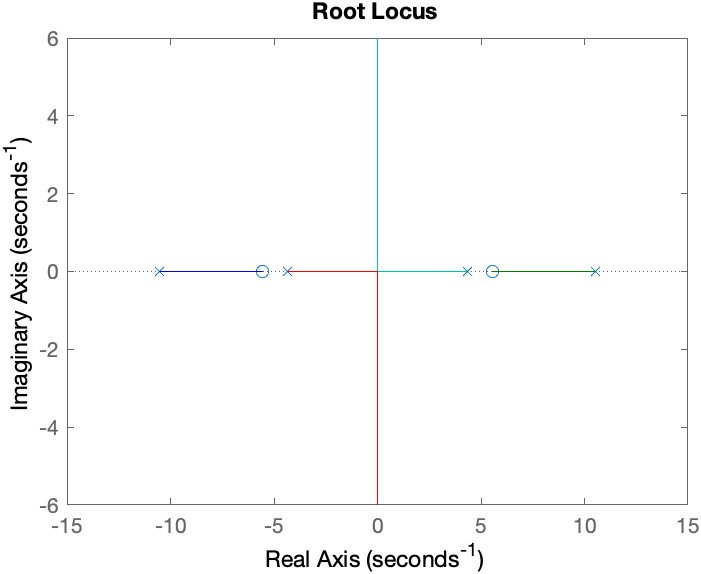
\includegraphics[height=200px]{../matlab/output/p4/y2_root-locus}
	\caption{Root locus of the two-rod plant}
	\label{fig:2rod:rl}
\end{figure}

Similar to \Cref{sec:4ai}, we would compute the overshoot $y_{os}$ bound curve based on the most sever pole at the far right side ($s=10.52$). After laying over against the one-rod system (in blue), as shown in \Cref{fig:2rod:os}, we may see the overshoot bound for two-rod plant is much sever than the one-rod. As a result the two-rod system needs a much faster system to control. 
\begin{figure}[H]
	\centering
	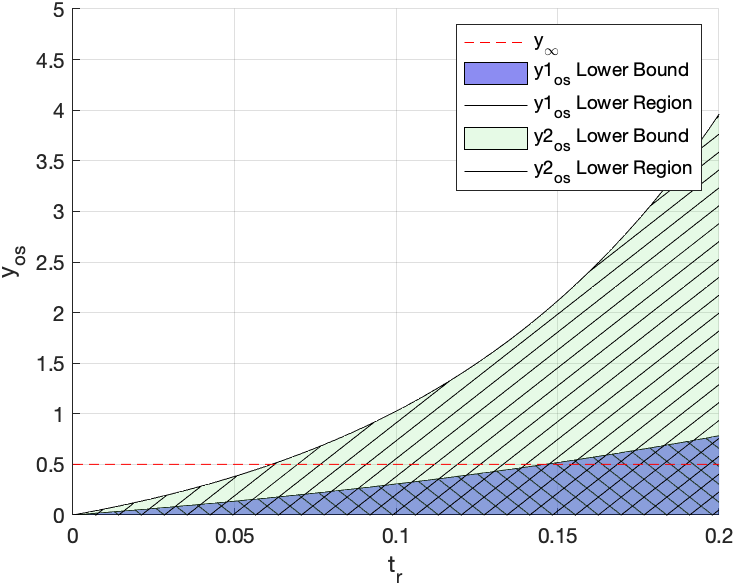
\includegraphics[height=200px]{../matlab/output/p4/y2_os-bound}
	\caption{Overshoot bound curve ($y1_{os}$: one-rod, $y2_{os}$: two-rod) vs. rise time}
	\label{fig:2rod:os}
\end{figure}

However, it is also not ideal to have a too fast system, since, the unstable zero needs a slower system to minimize the undershoot, as shown in \Cref{fig:2rod:us}.
\begin{figure}[H]
	\centering
	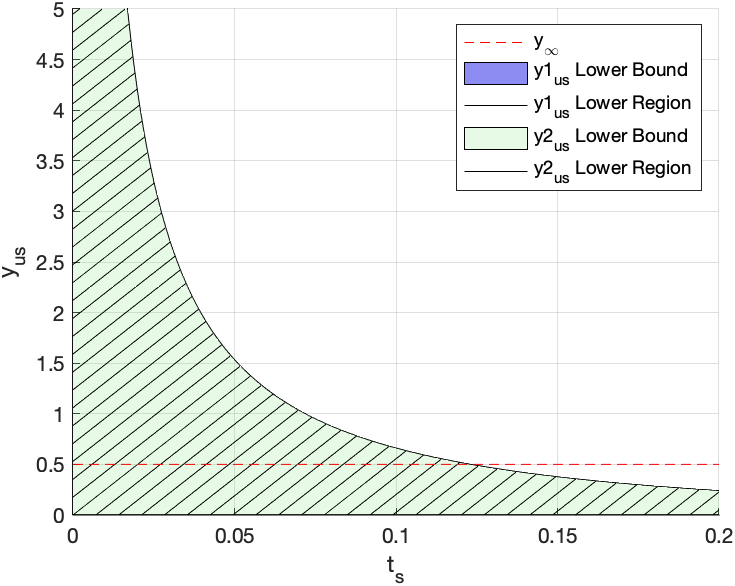
\includegraphics[height=200px]{../matlab/output/p4/y2_us-bound}
	\caption{Undershoot bound curve ($y1_{us}=0$: one-rod, $y2_{us}$: two-rod) vs. settling time}
	\label{fig:2rod:us}
\end{figure}

As a result, the two-rod system is more difficult to control than the one-rod system, since the two-rod system would have to suffer either or both severe undershoot and overshoot, whereas, the one-rod system can achieve simply by making the system faster.

Now, let's compute a meaningful bound on overshoot for the two-rod system using (1) on page 161. We may realize the sever pole results a negative bound which is meaningless, and the less sever pole results a positive bound of $3.5853$.

\begin{align}
	y2_{os}^{severe-pole} & = \frac{p}{z - p} = -2.112 \\
	y2_{os}^{moderate-pole} & = \frac{p}{z - p} = 3.5853
\end{align}

%\TODO{How does this bound compare to the bounds in your plots?}
Since the pg161 equation is only insightful for $p>z$, and in our case, we only know the fact that the transient performance is considerably pretty bad for the meaningful pole, since the pole and zero is close to each other. In addition, there exists a pole that is on right side of zero, resulting a negative overshoot, indicating, the situation is hopeless, and we would expect a pretty bad system. This bound tells us a combined effects of unstable zeros and poles, whereas the curve bounds tell us more insight about how the overshoot bound changes depending on rise time. Both bounds are telling us how bad this system is, but from two different perspectives.
d

\newpage
% --- ANS (a:ii) --- %
\subsubsection{(ii) $\Omega$ bound with \Gls{BSI}}
% Use the BSI to derive a lower bound on Ω. Comparing your answer to that in Problem P4(a)(ii)
% can we conclude that the two-rod system is definitely more difficult to control than the one-rod system?
Similar to \Cref{sec:4aii}, we may derive the lower bound on $\Omega$ from \Gls{BSI}, using the formulation of \Cref{eqn:omega:bnd}. As a result, we get a lower bound of $81.55 \unit{rad/s}$. As expected, the effects of double unstable more severe poles result the system needs a much larger positive region to compensate the reduced sensitivity in the low frequency region.

\begin{align}
	\Omega & \geq \frac{\pi * (4.3310 + 10.5200) - 0.1 * \ln(0.1)}{\ln(1.7783)} + 0.1 = 81.55 \unit{rad/s}\\
	\therefore\quad \Omega & \geq 81.55 \unit{rad/s}
\end{align}

As a result, we may conclude, the two-rod system is definitely more difficult to control, since it requires increased width of high frequency regions with increasing sensitivity to stabilize the system nicely.

% --- ANS (a:iii) --- %
\subsubsection{(iii) Poisson Integral}
% Repeat (ii) above, but this time try using the Poisson Integral instead of the BSI. In particular, use the Poisson Integral to show that, for the two-rod aiming system, it is impossible to satisfy the three design specifications given above.
Since there exists a real \Gls{ORHP} zero at $s=5.539$, hence the \Gls{PoI} holds, as a result we may derive a sensitivity boundary function. 

Let's assume the max peak sensitivity in the positive region of the Poisson Integral is $M = \underset{0.1<\omega<\Omega}{\max}|S(j\omega)|$. For simplicity, we let $\epsilon = \underset{\omega \in [0, 0.1]}{\max}|S(j\omega)|$.

We may now derive an relationship of the $M$ relative to the choice of attenuation frequency $\Omega$:
\begin{align}
	\int_0^{\infty} \ln |S(j\omega)| W(\omega) d\omega 	& = \pi \cdot \sum_{i=1}^{N_p} \ln |\frac{p_i + z}{p_i^* - z}| \\
\text{\Cref{spec:shut} \& \Cref{spec:track}} \Rightarrow \quad 	\int_0^{0.1} \ln |S(j\omega)| W(\omega) d\omega + \int_{0.1}^{\Omega} \ln |S(j\omega)| W(\omega) d\omega & \geq \pi \cdot \sum_{i=1}^{N_p} \ln |\frac{p_i + z}{p_i^* - z}| \\
\text{\Cref{spec:track}} \Rightarrow \quad 	\ln \{\underset{\omega \in [0, 0.1]}{\max}|S(j\omega)|\} \int_0^{0.1} W(\omega) d\omega + \ln \{\underset{\omega \in [0, 0.1]}{\max}|S(j\omega)|\} \int_{0.1}^{\Omega} W(\omega) d\omega & \geq \pi \cdot \sum_{i=1}^{N_p} \ln |\frac{p_i + z}{p_i^* - z}|  \\
\ln (\epsilon) \int_0^{0.1} W(\omega) d\omega + \ln(M) \int_{0.1}^{\Omega} W(\omega) d\omega & \geq \pi \cdot \sum_{i=1}^{N_p} \ln |\frac{p_i + z}{p_i^* - z}|  \\
\ln (\epsilon) \left[ 2 \tan^{-1} (\frac{\omega}{z})\right]_{0}^{0.1}+ \ln(M) \left[ 2 \tan^{-1} (\frac{\omega}{z})\right]_{0.1}^{\Omega} & \geq \pi \cdot \sum_{i=1}^{N_p} \ln |\frac{p_i + z}{p_i^* - z}| 
\end{align}

After rearrange:
\begin{align}
	\left[ 2 \tan^{-1} (\frac{\omega}{z})\right]_{0.1}^{\Omega} \geq 0 \Rightarrow \quad  \ln(M)  & \geq \frac{ \pi \cdot \sum_{i=1}^{N_p} \ln |\frac{p_i + z}{p_i^* - z}| -  \ln (\epsilon) \left[ 2 \tan^{-1} (\frac{\omega}{z})\right]_{0}^{0.1} }{ \left[ 2 \tan^{-1} (\frac{\omega}{z})\right]_{0.1}^{\Omega} } \\
	\ln(M)  & \geq \ln(M)\frac{ \pi \cdot \sum_{i=1}^{N_p} \ln |\frac{p_i + z}{p_i^* - z}| -  \ln (\epsilon) \left[ \tan^{-1} (\frac{0.1}{z})\right] }{ \left[ \tan^{-1} (\frac{\Omega}{z})\right] - \left[ \tan^{-1} (\frac{0.1}{z})\right] }\\
	\ln(M)  & \geq \frac{10.266}{\tan^{-1}\left(0.18054\,\Omega \right)-0.018052} \label{eqn:M-bound}
\end{align}

As a result, we can now plot the boundary equation \Cref{eqn:M-bound}, and overlay the max peak requirement from \Cref{spec:max}:
\begin{figure}[H]
	\centering
	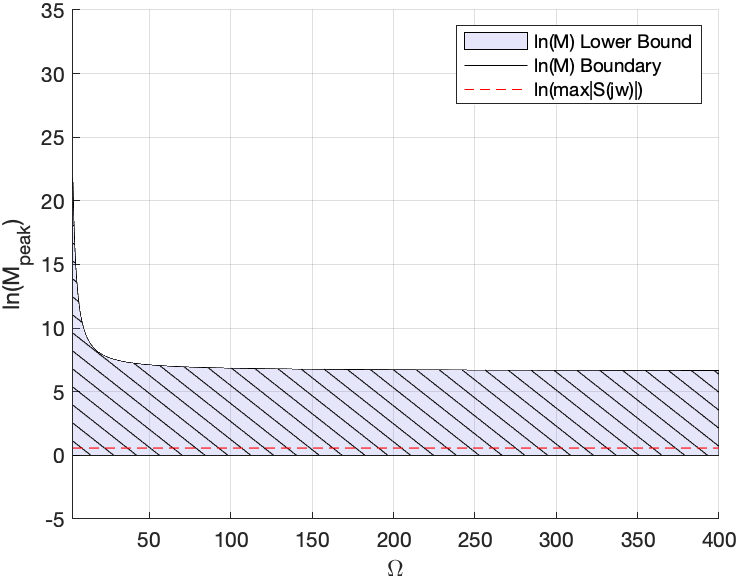
\includegraphics[height=200px]{../matlab/output/p4/M-bound}
	\caption{M peak bound vs. $\Omega$}
	\label{fig:2rod:m-peak}
\end{figure}

From the plot in \Cref{fig:2rod:m-peak}, we may find that no matter how we increase the attenuating frequency $\Omega$, the peak of the high frequency region would exceed the max peak sensitivity requirement (\Cref{spec:max}). As \Cref{eqn:M-bound-infinity} suggested, we may find the fact that $\ln(M(\Omega))\gg \ln(\epsilon)\, \forall \Omega$. 

\begin{equation}
\underset{\Omega \rightarrow \infty}{\ln(M)}  \geq \frac{10.266}{\tan^{-1}\left(0.18054\,(\Omega\rightarrow \infty) \right)-0.018052} = \frac{10.266}{ \pi / 2 - 0.018052} = 6.6115 \gg \ln(\epsilon) = 0.5756 \label{eqn:M-bound-infinity}
\end{equation}

In short, we can conclude it is impossible to satisfy the three design specifications given in \Cref{spec:track}, \Cref{spec:max}, and \Cref{spec:shut}.

%%%%%%%%%%%%%%%%%%%%%%%%%%%%%%%%%%%%%%%%%%%%%%%%%%%%%%%%%%%%%%%%%%%%%%%%%%%%%%%%
%% ************************************************************************** %%
%% *                      TODO [Remove For Final Copy!]                     * %%
%% ************************************************************************** %%
%%%%%%%%%%%%%%%%%%%%%%%%%%%%%%%%%%%%%%%%%%%%%%%%%%%%%%%%%%%%%%%%%%%%%%%%%%%%%%%%
%\printlistoftodos

%%%%%%%%%%%%%%%%%%%%%%%%%%%%%%%%%%%%%%%%%%%%%%%%%%%%%%%%%%%%%%%%%%%%%%%%%%%%%%%%
%% ************************************************************************** %%
%% *                                Glossary                                * %%
%% ************************************************************************** %%
%%%%%%%%%%%%%%%%%%%%%%%%%%%%%%%%%%%%%%%%%%%%%%%%%%%%%%%%%%%%%%%%%%%%%%%%%%%%%%%%
\clearpage
\printglossaries

%%%%%%%%%%%%%%%%%%%%%%%%%%%%%%%%%%%%%%%%%%%%%%%%%%%%%%%%%%%%%%%%%%%%%%%%%%%%%%%%
%% ************************************************************************** %%
%% *                               References                               * %%
%% ************************************************************************** %%
%%%%%%%%%%%%%%%%%%%%%%%%%%%%%%%%%%%%%%%%%%%%%%%%%%%%%%%%%%%%%%%%%%%%%%%%%%%%%%%%

% \printbibliography[heading=none]

%%%%%%%%%%%%%%%%%%%%%%%%%%%%%%%%%%%%%%%%%%%%%%%%%%%%%%%%%%%%%%%%%%%%%%%%%%%%%%%%
%% ************************************************************************** %%
%% *                               Appendices                               * %%
%% ************************************************************************** %%
%%%%%%%%%%%%%%%%%%%%%%%%%%%%%%%%%%%%%%%%%%%%%%%%%%%%%%%%%%%%%%%%%%%%%%%%%%%%%%%%
% appendices use section and subsection numbering
%\clearpage
\appendix
\begin{appendices}
% INPUT UR APPENDIX
\section{Code for Main}
\lstinputlisting[language=MATLAB, caption=Main Lab Contents, label=code:main]{../matlab/main_p3p4.m}


\section{Code for Helper Class}
\lstinputlisting[language=MATLAB, caption=Helper and commonly used functions by main, label=code:helper]{../matlab/helper.m}

\end{appendices}

\end{document}


